% https://tex.stackexchange.com/questions/204896/tikz-draw-line-thickness-less-than-0-1-mm/204897#204897x
\documentclass{article}
\usepackage{siunitx}
\usepackage{tikz}

\begin{document}

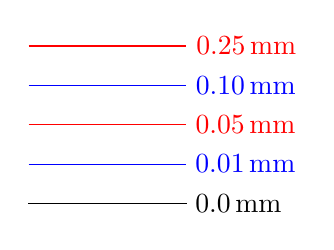
\begin{tikzpicture}[yscale=0.5]
    \draw [line width=0.25mm, red ] (0,-1) -- (2,-1) node [right] {\SI{0.25}{\milli\meter}};;
    \draw [line width=0.1mm,  blue] (0,-2) -- (2,-2) node [right] {\SI{0.10}{\milli\meter}};;
    \draw [line width=0.05mm, red ] (0,-3) -- (2,-3) node [right] {\SI{0.05}{\milli\meter}};
    \draw [line width=0.01mm, blue] (0,-4) -- (2,-4) node [right] {\SI{0.01}{\milli\meter}};
    \draw [line width=0mm,   black] (0,-5) -- (2,-5) node [right] {\SI{0.0}{\milli\meter}};
\end{tikzpicture}

\end{document}